\documentclass[12pt,a4paper]{report}

% ============================================================
% PACKAGES
% ============================================================
\usepackage[utf8]{inputenc}
\usepackage[T1]{fontenc}
\usepackage{mathptmx}               % Times-like font
\usepackage{geometry}
\usepackage{hyperref}
\usepackage{amsmath,amssymb}
\usepackage{graphicx}
\usepackage{booktabs}
\usepackage{tabularx}
\usepackage{longtable}
\usepackage{multirow}
\usepackage[table,xcdraw]{xcolor}
\usepackage{titlesec}
\usepackage{setspace}
\usepackage{caption}
\usepackage{subcaption}
\usepackage{tocloft}
\usepackage{fancyhdr}
\usepackage{enumitem}
\usepackage{listings}
\usepackage{microtype}
\usepackage{array}
\usepackage{float}
\usepackage{mdframed}
\usepackage{tikz}
\usetikzlibrary{positioning, arrows.meta, fit}
\usepackage{parskip}
\usepackage{afterpage}
\usepackage{eso-pic}
\usepackage{etoolbox}
\usepackage{chngpage}

% ============================================================
% GEOMETRY SETUP FOR FRONT MATTER
% ============================================================
\newgeometry{left=1.5cm, right=1.5cm, top=2cm, bottom=2cm}

% ============================================================
% COLORS
% ============================================================
\definecolor{sectionblue}{RGB}{0,70,127}
\definecolor{tablebala}{RGB}{0,70,127}
\definecolor{tablerowodd}{RGB}{235,242,250}
\definecolor{codebackground}{RGB}{248,248,248}
\definecolor{codeborder}{RGB}{180,180,180}
\definecolor{noteblue}{RGB}{220,235,250}

% ============================================================
% HYPERREF SETUP
% ============================================================
\hypersetup{
    colorlinks=true,
    linkcolor=sectionblue,
    urlcolor=sectionblue,
    citecolor=sectionblue,
    pdfauthor={Aditya K, P Akshay, Punarvi M U, Rakshith H N},
    pdftitle={Project Report: Autonomous AI Agent for SOC Triage and Forensic Investigation}
}

% ============================================================
% SECTION FORMATTING - CHAPTERS LEFT ALIGNED
% ============================================================
\titleformat{\chapter}[display]
  {\normalfont\Large\bfseries}  % Removed \centering
  {\chaptertitlename\ \thechapter}{0pt}{\Large}
\titlespacing*{\chapter}{0pt}{-20pt}{10pt}

\titleformat{\section}
  {\normalfont\fontsize{14}{17}\bfseries\color{sectionblue}}
  {\thesection}{1em}{}

\titleformat{\subsection}
  {\normalfont\fontsize{12}{15}\bfseries\color{sectionblue}}
  {\thesubsection}{1em}{}

\titleformat{\subsubsection}
  {\normalfont\fontsize{11}{14}\bfseries\itshape}
  {\thesubsubsection}{1em}{}

\titlespacing*{\section}{0pt}{16pt}{8pt}
\titlespacing*{\subsection}{0pt}{12pt}{6pt}
\titlespacing*{\subsubsection}{0pt}{10pt}{4pt}

% ============================================================
% HEADER / FOOTER FOR MAIN CONTENT (Chapter 1 onwards)
% ============================================================
\fancypagestyle{mainstyle}{
  \fancyhf{}
  \fancyhead[L]{\small\textbf{Autonomous AI Agent for SOC Triage and Forensic Investigation}}
  \fancyhead[R]{}
  \fancyfoot[L]{\small Dept. of ISE}
  \fancyfoot[C]{\small 2025-26}
  \fancyfoot[R]{\small \thepage}
  \renewcommand{\headrulewidth}{0.5pt}
  \renewcommand{\footrulewidth}{0.5pt}
}

% Plain style for chapter pages (using same header/footer)
\fancypagestyle{plain}{
  \fancyhf{}
  \fancyhead[L]{\small\textbf{Autonomous AI Agent for SOC Triage and Forensic Investigation}}
  \fancyhead[R]{}
  \fancyfoot[L]{\small Dept. of ISE}
  \fancyfoot[C]{\small 2025-26}
  \fancyfoot[R]{\small \thepage}
  \renewcommand{\headrulewidth}{0.5pt}
  \renewcommand{\footrulewidth}{0.5pt}
}

% ============================================================
% CAPTION STYLE
% ============================================================
\captionsetup[figure]{
  labelfont={bf,color=sectionblue},
  textfont=it,
  labelsep=period,
  justification=centering,
  font=small
}
\captionsetup[table]{
  labelfont={bf,color=sectionblue},
  textfont=it,
  labelsep=period,
  justification=centering,
  font=small,
  position=top
}

% ============================================================
% TABLE STYLE HELPER
% ============================================================
\newcommand{\tblhead}[1]{\cellcolor{tableheader}\color{white}\textbf{#1}}
\newcommand{\hcell}[1]{\cellcolor{tableheader}\color{white}\textbf{#1}}

% ============================================================
% NOTE BOX
% ============================================================
\newmdenv[
  backgroundcolor=noteblue,
  linecolor=sectionblue,
  linewidth=1pt,
  innerleftmargin=10pt,
  innerrightmargin=10pt,
  innertopmargin=8pt,
  innerbottommargin=8pt,
  skipabove=8pt,
  skipbelow=8pt
]{notebox}

% ============================================================
% SPACING
% ============================================================
\setlength{\parskip}{4pt}
\setlength{\parindent}{0pt}
\onehalfspacing

% ============================================================
% PREVENT PAGE BREAK IN REFERENCES
% ============================================================
\makeatletter
\patchcmd{\thebibliography}{\chapter*}{\section*}{}{}
\makeatother

% ============================================================
% PAGE BORDER COMMAND
% ============================================================
\newcommand\pageborder{%
    \begin{tikzpicture}[remember picture, overlay, inner sep=0]
        \draw[line width=0.8pt] 
            ([xshift=0.5cm,yshift=-0.5cm]current page.north west) 
            rectangle 
            ([xshift=-0.5cm,yshift=0.5cm]current page.south east);
    \end{tikzpicture}%
}

% ============================================================
% TURN ON BORDER FOR FRONT MATTER
% ============================================================
\AddToShipoutPicture*{\pageborder}

\begin{document}

% ========== FRONT MATTER PAGES (WITH BORDER, NO HEADER/FOOTER) ==========

% ========== TITLE PAGE ==========
\begin{titlepage}
  \begin{center}
    {\large\bfseries VISVESVARAYA TECHNOLOGICAL UNIVERSITY}\\[2pt]
    {\small "JNANA SANGAMA", BELAGAVI -- 590\,018}\\[8pt]
    \rule{\linewidth}{0.6pt}

    \vfill
    \includegraphics[width=3.5cm]{VTU-Logo-250x250-1.png}

    \vfill

    {\Large\bfseries Major Project Phase 1 Report (BIS685)}\\[10pt]
    \rule{0.6\linewidth}{0.4pt}\\[8pt]
    {\Large\bfseries An Autonomous Terminal-Based AI Agent for SOC Triage} \\[8pt]
    {\Large\bfseries and Forensic Investigation}

    \vfill

    {\large\itshape submitted in partial fulfilment of the requirement for the award of the degree of}\\[6pt]
    {\Large\bfseries BACHELOR OF ENGINEERING}\\[2pt]
    {\large\itshape in}\\[4pt]
    {\Large\bfseries INFORMATION SCIENCE AND ENGINEERING}

    \vfill

    {\large\bfseries Submitted By}\\[8pt]
    \begin{tabular}{@{}ll@{}}
      \textbf{Aditya K}          & \texttt{1MP23IS003} \\
      \textbf{P Akshay}          & \texttt{1MP23IS038} \\
      \textbf{Punarvi M U}       & \texttt{1MP23IS042} \\
      \textbf{Rakshith H N}      & \texttt{1MP23IS043} \\
    \end{tabular}

    \vfill

    \begin{minipage}{0.48\textwidth}
      \centering
      \textbf{Under the guidance of}\\[6pt]
      \textbf{Mrs. Jyothi R}\\
      {\small Assistant Professor, Dept. of ISE}
    \end{minipage}

    \vfill

    \includegraphics[width=3.5cm]{bgscet_logo-removebg-preview.png}\\[4pt]
    {\large\bfseries BGS COLLEGE OF ENGINEERING AND TECHNOLOGY}\\
    {\small CA Site No. 6 \& 7, 3rd Main, Pipeline Road, Chord Rd,\\
     Mahalakshmipuram, Bengaluru, Karnataka -- 560086}\\[4pt]
    {\large\bfseries 2025 -- 2026}
  \end{center}
\end{titlepage}

% ========== CERTIFICATE PAGE ==========
\newpage
\thispagestyle{empty}
\begin{center}
  \textit{\textbf{|| Jai Sri Gurudev ||}} \\[2pt]
  \textbf{Sri Adichunchanagiri Shikshana Trust} \\[4pt]
    {\large\bfseries BGS COLLEGE OF ENGINEERING AND TECHNOLOGY}\\
      Mahalakshmipuram, West of Chord Road, Bengaluru -- 560 086\\[2pt]
  \includegraphics[width=1.2in]{bgscet_logo-removebg-preview.png}\\[4pt]
{\large\bfseries\textcolor{red}{DEPARTMENT OF INFORMATION SCIENCE AND ENGINEERING}}
\end{center}

\vspace{0.3cm}
\begin{center}
  \underline{\textbf{CERTIFICATE}}
\end{center}

\noindent
Certified that the dissertation entitled \textbf{``An Autonomous Terminal-Based AI Agent for SOC Triage and Forensic Investigation''} carried out by \textbf{Aditya K (1MP23IS003), P Akshay (1MP23IS038), Punarvi M U (1MP23IS042), Rakshith H N (1MP23IS043)} are bonafide students of \textbf{BGS College of Engineering and Technology} in partial fulfilment for the award of \textbf{``BACHELOR OF ENGINEERING''} in \textbf{Information Science and Engineering} under \textbf{VISVESVARAYA TECHNOLOGICAL UNIVERSITY, BELAGAVI} during the academic year \textbf{2025--26}. It is certified that all corrections indicated for internal assessment have been incorporated in the report deposited in the departmental library. The project report has been approved as it satisfies the academic requirements in respect of project work prescribed for the said degree.

\vspace{0.8cm}

\begin{minipage}[t]{0.45\textwidth}
  \textbf{Mrs. Jyothi R}\\
  Guide\\
  Assistant Professor, Dept. of ISE
\end{minipage}
\hfill
\begin{minipage}[t]{0.45\textwidth}
  \textbf{Signature of Guide}
\end{minipage}

\vspace{0.6cm}

\begin{minipage}[t]{0.45\textwidth}
  \textbf{Dr. Chaitra Naveen}\\
  Head of Department\\
  Dept. of ISE
\end{minipage}
\hfill
\begin{minipage}[t]{0.45\textwidth}
  \textbf{Signature of HOD}
\end{minipage}

\vspace{0.6cm}

\begin{minipage}[t]{0.45\textwidth}
  \textbf{Dr. RaviKumar G K}\\
  Principal\\
  BGS College of Engineering \& Technology
\end{minipage}
\hfill
\begin{minipage}[t]{0.45\textwidth}
  \textbf{Signature of Principal}
\end{minipage}

\vspace{0.6cm}

\begin{minipage}[t]{0.45\textwidth}
  \textbf{External Examiner}
\end{minipage}
\hfill
\begin{minipage}[t]{0.45\textwidth}
  \textbf{Signature of External Examiner}
\end{minipage}

\vspace{0.8cm}
\begin{center}
  Place: Bengaluru\\
  Date:
\end{center}

% ========== DECLARATION PAGE ==========
\newpage
\thispagestyle{empty}
\begin{center}
  \textit{\textbf{|| Jai Sri Gurudev ||}} \\[2pt]
  \textbf{Sri Adichunchanagiri Shikshana Trust} \\[4pt]
    {\large\bfseries BGS COLLEGE OF ENGINEERING AND TECHNOLOGY}\\
      Mahalakshmipuram, West of Chord Road, Bengaluru -- 560 086\\[2pt]
  \includegraphics[width=1.2in]{bgscet_logo-removebg-preview.png}\\[4pt]
{\large\bfseries\textcolor{red}{DEPARTMENT OF INFORMATION SCIENCE AND ENGINEERING}}
\end{center}

\vspace{0.3cm}
\begin{center}
  \underline{\textbf{DECLARATION BY THE STUDENTS}}
\end{center}

\noindent
We, \textbf{Aditya K (1MP23IS003), P Akshay (1MP23IS038), Punarvi M U (1MP23IS042), Rakshith H N (1MP23IS043)} students of VI semester Information Science and Engineering Department, \textbf{BGS COLLEGE OF ENGINEERING \& TECHNOLOGY}, hereby declare that the dissertation for the project entitled \textbf{``An Autonomous Terminal-Based AI Agent for SOC Triage and Forensic Investigation''} submitted to the \textbf{Visvesvaraya Technological University, Belagavi} during the academic year 2025-2026, is a record of an original work done by us under the guidance of our internal guide \textbf{Mrs. Jyothi R, Assistant Professor}, Department of Information Science and Engineering, BGS College of Engineering \& Technology, Bengaluru. This dissertation is submitted in partial fulfilment for the award of Bachelor of Engineering in Information Science and Engineering. The results embodied in this report have not been submitted to any other University or Institute for the award of any degree.

\vspace{0.8cm}

\noindent
\begin{tabular}{@{}p{0.55\textwidth}@{}p{0.4\textwidth}@{}}
  \textbf{Aditya K [1MP23IS003]} & \underline{\hspace{3cm}} \\
  & \textbf{Signature} \\[0.8cm]
  \textbf{P Akshay [1MP23IS038]} & \underline{\hspace{3cm}} \\
  & \textbf{Signature} \\[0.8cm]
  \textbf{Punarvi M U [1MP23IS042]} & \underline{\hspace{3cm}} \\
  & \textbf{Signature} \\[0.8cm]
  \textbf{Rakshith H N [1MP23IS043]} & \underline{\hspace{3cm}} \\
  & \textbf{Signature} \\
\end{tabular}

% ========== ACKNOWLEDGEMENT PAGE ==========
\newpage
\begin{center}
  {\Large\bfseries ACKNOWLEDGEMENT}
\end{center}
\vspace{0.5cm}
\thispagestyle{empty}
\addcontentsline{toc}{chapter}{Acknowledgement}

We bow in deep reverence and gratitude to His Divine Soul \textbf{Jagadguru Padmabhushan Sri Sri Sri Dr. Balagangadharanatha Mahaswamiji} and His Holiness \textbf{Jagadguru Sri Sri Sri Dr. Nirmalanandanatha Mahaswamiji}, whose divine grace and blessings have enabled us to pursue and successfully complete our academics in this esteemed institution.

We would also like to express our humble gratitude to \textbf{Sri. Sri. Soumyanatha Swamiji} for his blessings and encouragement, which have been a source of inspiration in our academic journey.

We wish to express our deep sincere feelings of gratitude to our institution, \textbf{BGS College of Engineering \& Technology}, for providing an opportunity for completing our Project work successfully.

We would also like to express our deep sense of gratification to \textbf{Dr. Raju G T}, Director, BGS College of Engineering \& Technology, for his continuous support in providing amenities to carry out this Project work in this admired institution.

We express our deep appreciation to \textbf{Dr. RaviKumar G K}, Principal, BGS College of Engineering \& Technology, for providing us with excellent facilities and academic ambience; which have helped us in satisfactory completion of Project work.

We extend our sincere thanks to \textbf{Dr. Chaitra Naveen}, Head of the Department, Information Science and Engineering for providing us an invaluable support throughout the period of our Project work.

We wish to express our heartfelt gratitude to our Project Coordinator \textbf{Mrs. Jyothi R}, Assistant Professor, Department of ISE for her valuable guidance, suggestions and cheerful encouragement during the entire period of our Project work.

We extend our heartfelt thanks to our guide \textbf{Mrs. Jyothi R} for her expert guidance, patience, and motivation, which helped us in completing this work effectively.

Finally, we take this opportunity to extend our earnest gratitude and respect to our parents, Teaching \& Non-teaching staff of the department, the library staff and all our friends, who have directly or indirectly supported us during the period of our Project work.

\vspace{0.5cm}

\begin{flushright}
  \textbf{Regards,} \\
  \textbf{Aditya K} \quad [1MP23IS003] \\
  \textbf{P Akshay} \quad [1MP23IS038] \\
  \textbf{Punarvi M U} \quad [1MP23IS042] \\
  \textbf{Rakshith H N} \quad [1MP23IS043]
\end{flushright}

% ========== ABSTRACT PAGE ==========
\newpage
\begin{center}
  {\Large\bfseries ABSTRACT}
\end{center}
\vspace{0.5cm}
\thispagestyle{empty}
\addcontentsline{toc}{chapter}{Abstract}

This project presents the design and development of an autonomous terminal-based AI agent for Security Operations Center (SOC) triage and forensic investigation. The proposed system leverages locally deployed Large Language Models (LLMs) – specifically DeepSeek-R1 and Llama 3.3 (70B) – to replicate and enhance the decision-making capabilities of a Tier~1 SOC analyst. By integrating real-time threat detection using CNN/LSTM models (accuracy >95\%), explainable AI via SHAP and LIME, and automated memory/disk forensics using Volatility3 and Autopsy-CLI, the agent provides a unified pipeline from alert ingestion to root cause analysis. A natural language chat interface allows analysts to query alerts and investigations in plain English. All components run on-premises, ensuring data privacy and eliminating third‑party API dependencies. Expected outcomes include a reduction of false positives from >90\% to <10\%, a 90\% decrease in alert processing time, and a 70\% reduction in analyst workload for routine triage tasks.

\vspace{0.3cm}
\noindent
\textbf{Keywords:} SOC automation, LLM agents, explainable AI, digital forensics, cybersecurity, threat detection.

% ========== VISION AND MISSION (INSTITUTE) ==========
\newpage
\begin{center}
  {\Large\bfseries Vision and Mission of the Institute}
\end{center}
\vspace{0.5cm}
\thispagestyle{empty}
\addcontentsline{toc}{chapter}{Vision and Mission of the Institute}

\section*{\textit{Vision}}
Creating Competent IT Professionals with Core Values for the Real World.

\section*{\textit{Mission}}
\begin{itemize}
  \item Providing Students with a Sound Knowledge in IT Fundamentals.
  \item Exposing Students to Emerging Frontiers in various domains of IT enabling Continuous Learning.
  \item Promoting Excellence in Teaching, Training, Research and Consultancy.
  \item Developing Entrepreneurial acumen to venture into Innovative areas of IT.
  \item Imparting value based Professional Education with a sense of Social Responsibility.
\end{itemize}

% ========== VISION AND MISSION (DEPARTMENT) ==========
\newpage
\begin{center}
  {\Large\bfseries Vision and Mission of the Department}
\end{center}
\vspace{0.5cm}
\thispagestyle{empty}
\addcontentsline{toc}{chapter}{Vision and Mission of the Department}

\section*{\textit{Vision}}
To excel in teaching and innovative research in the field of information science and engineering to support technologically globalized society.

\section*{\textit{Mission}}
\begin{itemize}
  \item To inculcate strong academic foundation in the information technology domain to empower and equip students for successful career through various teaching learning approaches.
  \item To identify innovative research-based activities and strengthen entrepreneurial abilities.
  \item To emphasize the ethical use of technology instilling in our students, a sense of social responsibility towards the betterment of society.
\end{itemize}

% ========== TABLE OF CONTENTS ==========
\newpage
\renewcommand{\contentsname}{Table of Contents}
\tableofcontents
\thispagestyle{empty}

% ========== TURN OFF BORDER FOR MAIN CONTENT ==========
\AddToShipoutPicture*{}

% ========== RESET GEOMETRY AND PAGE NUMBERING FOR MAIN CONTENT ==========
\newgeometry{left=1.5cm, right=1.5cm, top=2cm, bottom=2cm}
\clearpage
\pagenumbering{arabic}
\pagestyle{mainstyle}

% ============================================================
% MAIN REPORT (Chapter 1 onwards with header/footer, NO border)
% ============================================================

\chapter{Introduction}

\section{Significance of the Project}

\subsection{The Current State of Security Operations Centers}
Security Operations Centers (SOCs) serve as the centralized defense units within modern organizations, responsible for continuous monitoring, detection, analysis, and response to cyber threats. These centers operate with a tiered analyst structure where Tier~1 analysts—typically the least experienced—perform the critical function of initial alert triage. According to Vielberth et al.~\cite{vielberth2020}, SOCs generate thousands of alerts daily, with false positive rates often exceeding 90\%. This means that fewer than 10 of every 100 alerts represent actual threats, while the rest consume valuable analyst time.

\subsection{The Cybersecurity Workforce Crisis}
Furnell~\cite{furnell2021} reports between 1.8~million and 4~million unfilled cybersecurity positions worldwide. Sundaramurthy et al.~\cite{sundaramurthy2015} documented annual turnover rates of 30--40\% in SOCs due to burnout from repetitive, high-stress tasks. Automating routine triage can reduce burnout and allow analysts to focus on higher-value work.

\subsection{Opportunity for AI-Powered SOC Automation}
Recent advances in Large Language Models (LLMs) present unprecedented opportunities. Zhao et al.~\cite{zhao2023} note that modern LLMs possess emergent abilities including in-context learning, chain-of-thought reasoning, and instruction following. Oniagbi~\cite{oniagbi2024} empirically validated that LLM agents can achieve 100\% recall and 91.4\% accuracy for SOC Tier~1 triage using models like GPT-4o and Llama~3~70B.

\subsection{Gaps Addressed by this Project}
Despite these advances, existing systems lack explainability, raise privacy concerns (third-party APIs), and keep detection and forensics fragmented. This project addresses these gaps by developing an autonomous terminal-based AI agent that uniquely combines:
\begin{itemize}
    \item LLM reasoning with locally deployed models
    \item Explainable AI (XAI) using SHAP and LIME
    \item Automated memory and disk forensics
    \item Natural language interaction for analysts
    \item Privacy preservation through local deployment
\end{itemize}

\section{Problem Statement}

SOC analysts are overwhelmed due to:
\begin{itemize}
    \item \textbf{Massive log volume:} SIEM platforms ingest terabytes daily, growing 10--15\% annually.
    \item \textbf{High false positive rates:} Exceeding 90\%, leading to alert fatigue.
    \item \textbf{Manual triage workflows:} Kersten et al.~\cite{kersten2023} identified a four-stage manual process that is time-consuming.
    \item \textbf{Lack of explainability:} Existing AI systems operate as black boxes, reducing trust.
    \item \textbf{Fragmented forensics:} Detection and investigation require manual handoffs, delaying response.
\end{itemize}

Consequences include missed threats, slow response (breach dwell time), analyst burnout, and regulatory risk.

\section{Research Motivation}

The motivation stems from three observations from the literature:
\begin{enumerate}
    \item \textbf{Capability-ready technology exists:} LLMs possess reasoning abilities that align perfectly with SOC triage~\cite{zhao2023,yao2024}.
    \item \textbf{Validated proof-of-concept exists:} Oniagbi~\cite{oniagbi2024} achieved 100\% recall and 91.4\% accuracy with LLM agents.
    \item \textbf{Clear path to improvement exists:} Limitations (lack of explainability, privacy, no unified forensics) have clear technical solutions.
\end{enumerate}
The project creates a unified solution that integrates LLM reasoning, XAI, forensics, continuous learning, natural language querying, and local deployment.

% ============================================================
% CHAPTER 2: LITERATURE REVIEW
% ============================================================
\chapter{Literature Review}

The literature survey examined over 25 peer-reviewed papers spanning SOC operations, LLM applications, XAI, threat detection, digital forensics, and autonomous agents.

\section{SOC Operations and Tier 1 Analyst Challenges}
Kersten et al.~\cite{kersten2023} proposed a four-stage triage model: (1) relevance indicators, (2) alert history, (3) related logs, (4) attacker information/IOCs. Vielberth et al.~\cite{vielberth2020} identified average analysis time and false positive rate as key SOC metrics. Ban et al.~\cite{ban2021} showed AI-assisted techniques reduce alert fatigue.

\section{Large Language Models in Cybersecurity}
Zhao et al.~\cite{zhao2023} surveyed LLM evolution and emergent abilities. Yao et al.~\cite{yao2024} identified four core capabilities: natural language comprehension, text generation, domain knowledge, instruction following. Motlagh et al.~\cite{motlagh2024} reviewed LLMs for anomaly detection and decision support. Kaheh et al.~\cite{kaheh2023} introduced ``Cyber Sentinel'' using GPT-4. Oniagbi~\cite{oniagbi2024} specifically evaluated LLM agents for SOC Tier~1 triage, achieving 100\% recall and 91.4\% accuracy with Llama~3~70B. Fang et al.~\cite{fang2024} demonstrated autonomous exploitation of one-day vulnerabilities. Wu et al.~\cite{wu2023} highlighted hallucination risks.

\section{Explainable AI (XAI) for Cybersecurity}
Salloum and Norozpour~\cite{salloum2025} proposed an XAI-IDS combining CNN with SHAP and LIME, achieving 94\% accuracy with interpretable outputs. Lundberg and Lee~\cite{lundberg2017} introduced SHAP for unified interpretation. Ribeiro et al.~\cite{ribeiro2016} developed LIME. Capuano et al.~\cite{capuano2022} surveyed XAI in cybersecurity. Calzarossa, Giudici, and Zieni~\cite{calzarossa2025} proposed an assessment framework using Lorenz curves and Gini coefficients.

\section{AI-Driven Threat Detection}
Ankalaki et al.~\cite{ankalaki2025} comprehensively reviewed AI methods for attack prediction. Rishad et al.~\cite{rishad2025} conducted a comparative study; results are summarised in Table~\ref{tab:model_comparison}. Al-Shurbaji et al.~\cite{alshurbaji2025} reviewed DL-based IDS for IoT botnets. Hiari et al.~\cite{hiari2025} achieved 99.92\% accuracy with refined LSTM for DoS detection.

\begin{table}[H]
\centering
\caption{Comparative Performance of AI/ML Models for Threat Detection (Source:~\cite{rishad2025})}
\small
\begin{tabular}{@{}lccccc@{}}
\toprule
\hcell{Model} & \hcell{Accuracy (\%)} & \hcell{Precision (\%)} & \hcell{Recall (\%)} & \hcell{AUC-ROC (\%)} \\
\midrule
Logistic Regression & 87.4 & 85.6 & 83.2 & 88.1 \\
Random Forest & 92.3 & 90.7 & 91.2 & 94.5 \\
XGBoost & 94.1 & 92.5 & 92.8 & 96.7 \\
CNN & 95.8 & 94.2 & 93.5 & 97.3 \\
LSTM & 94.7 & 93.3 & 92.6 & 96.8 \\
\bottomrule
\end{tabular}
\label{tab:model_comparison}
\end{table}

\section{Digital Forensics and Incident Response}
Ndihe~\cite{ndihe2024} presented AI-driven forensic systems for real-time anomaly detection. Kolluri~\cite{kolluri2016} proposed automated evidence collection. Kara~\cite{kara2023} examined fileless malware and memory forensics using Volatility. Rana~\cite{rana2025} discussed AI assistants like Microsoft Copilot for workflow automation.

\section{Autonomous Agents and Frameworks}
Fang et al.~\cite{fang2024} showed LLM agents can autonomously execute security tasks (87\% success on one-day exploits). Chen et al.~\cite{chen2024} noted that multi-agent architectures improve performance. Muzsai et al.~\cite{muzsai2024} introduced HackSynth with a Planner-Summarizer architecture. LangGraph and CrewAI enable state management and tool integration.

\section{Datasets and Evaluation Metrics}
Ankalaki et al.~\cite{ankalaki2025} catalogued datasets: NSL-KDD (125k records), CICIDS2017 (2.8M), UNSW-NB15 (2.5M), Bot-IoT (3.5M), CICIoT2023 (56k). Standard metrics include accuracy, precision, recall, F1-score, false positive rate (FPR), AUC-ROC, MTTD, and MTTR.

\section{Research Gap}
From the literature, the following gaps are identified:
\begin{table}[H]
\centering
\caption{Research Gaps Identified}
\begin{tabular}{@{}p{5.5cm}p{7cm}@{}}
\toprule
\hcell{Gap} & \hcell{Supporting Evidence} \\
\midrule
Limited LLM application in SOC triage & Motlagh et al.~\cite{motlagh2024} \\
Lack of explainability in detection & Salloum and Norozpour~\cite{salloum2025} \\
No unified detection-forensics pipeline & Ndihe~\cite{ndihe2024} \\
Static models with low adaptability & Vielberth et al.~\cite{vielberth2020} \\
No natural language interaction & Oniagbi~\cite{oniagbi2024} \\
Hallucination risks with LLMs & Wu et al.~\cite{wu2023} \\
Privacy concerns with third-party APIs & Oniagbi~\cite{oniagbi2024} \\
\bottomrule
\end{tabular}
\end{table}
The proposed system addresses all these gaps by integrating LLM reasoning, XAI, unified forensics, local deployment, and natural language interaction.

% ============================================================
% CHAPTER 3: OBJECTIVES
% ============================================================
\chapter{Objectives}

The main goal is to develop an autonomous terminal-based AI agent for SOC Tier~1 alert triage and forensic investigation that reduces false positives, provides explainable decisions, enables natural language interaction, and unifies detection, analysis, and forensics with local deployment.

Specific objectives:

\begin{enumerate}
    \item \textbf{Real-time threat detection:} Implement CNN/LSTM models for anomaly detection (accuracy >95\%, FPR <10\%).
    \item \textbf{Explainable AI:} Integrate SHAP and LIME for interpretable predictions. Every alert includes a human-readable explanation.
    \item \textbf{Forensic investigation module:} Use Volatility3 and Autopsy-CLI for memory/disk forensics; automated timeline reconstruction and root cause analysis within 5 minutes.
    \item \textbf{LLM reasoning engine:} Deploy DeepSeek-R1 and Llama~3.3~(70B) locally using Ollama/vLLM; implement chain-of-thought reasoning.
    \item \textbf{Natural language querying:} Terminal-based chat interface for plain-language questions about alerts and investigations.
    \item \textbf{Predictive capabilities:} Trend analysis to identify emerging threat patterns and generate proactive alerts.
\end{enumerate}

% ============================================================
% CHAPTER 4: PROPOSED SYSTEM
% ============================================================
\chapter{Proposed System}

\section{Methodology}

\subsection{System Architecture Overview}
The proposed Autonomous AI-Powered SOC Agent follows a modular architecture as illustrated below:

\begin{figure}[H]
\centering
\begin{tikzpicture}[
  node distance=0.5cm,
  box/.style={draw, rectangle, minimum width=11cm, minimum height=0.9cm, align=center, font=\small, rounded corners=2pt},
  titlebox/.style={draw, rectangle, minimum width=8cm, minimum height=0.7cm, align=center, font=\bfseries, rounded corners=2pt, fill=blue!20},
  arrow/.style={-{Stealth[scale=1.2]}, thick}
]
  % Title box
  \node[titlebox] (title) {Autonomous SOC Agent};
  
  % Main layers stacked vertically below title
  \node[box, below=0.6cm of title, fill=blue!10] (data) {Data Collection Layer --- Wazuh SIEM};
  \node[box, below=0.6cm of data, fill=blue!10] (threat) {Threat Detection Layer --- CNN/LSTM Models};
  \node[box, below=0.6cm of threat, fill=blue!10] (llm) {LLM Reasoning Layer --- DeepSeek-R1 / Llama 3.3};
  \node[box, below=0.6cm of llm, fill=blue!10] (forensic) {Forensic Module --- Volatility3 / Autopsy-CLI};
  
  % Side capabilities
  \node[draw, rectangle, minimum width=4cm, minimum height=0.7cm, align=center, font=\footnotesize, fill=gray!10, right=0.8cm of threat] (xai) {SHAP / LIME (XAI)};
  \node[draw, rectangle, minimum width=4cm, minimum height=0.7cm, align=center, font=\footnotesize, fill=gray!10, right=0.8cm of llm] (nlp) {Natural Language Interface};
  
  % Arrows
  \draw[arrow] (data) -- (threat);
  \draw[arrow] (threat) -- (llm);
  \draw[arrow] (llm) -- (forensic);
  \draw[arrow] (threat.east) -- (xai.west);
  \draw[arrow] (llm.east) -- (nlp.west);
  
  % Outer box
  \draw[thick, rounded corners=3pt] ($(title.north west)+(-0.4,0.3)$) rectangle ($(forensic.south east)+(0.5,-0.5)$);
\end{tikzpicture}
\caption{System Architecture Diagram}
\label{fig:architecture}
\end{figure}

\subsection{Data Collection Layer}
Integration with Wazuh SIEM/XDR for real-time alert ingestion, system logs via journalctl/osquery, network traffic via tshark/nmap, and threat intelligence feeds (AbuseIPDB, URLScan.io, AlienVault OTX).

\subsection{Threat Detection Layer}
CNN for network traffic pattern recognition (3 convolutional layers with 32,64,128 filters; max pooling; dense 128 ReLU; sigmoid output). LSTM for sequence-based anomaly detection (2 LSTM layers with 64 and 32 units; dropout 0.2; dense 16 ReLU; sigmoid output). Both achieve >95\% accuracy.

\subsection{Explainable AI Layer}
SHAP assigns each feature an importance value based on game theory. LIME generates local explanations by approximating the model with an interpretable surrogate. Every detection decision is accompanied by a human-readable justification.

\subsection{LLM Reasoning Layer}
Chain-of-Thought prompting breaks complex reasoning into steps: relevance indicators, alert history, log correlation, IOC extraction. Local models: DeepSeek-R1 (67B) for primary reasoning, Llama~3.3~(70B) for validation, Mistral Small 3.1/Phi-4 for fast parsing. Deployment via Ollama and vLLM ensures data never leaves the organization.

\subsection{Forensic Investigation Layer}
Memory forensics with Volatility3 (pslist, netscan, malfind, modscan) for fileless malware detection. Disk forensics with Autopsy-CLI. Automated timeline reconstruction normalises timestamps, sorts events, identifies attack sequences, and generates visual timelines with annotated events.

\subsection{Orchestration Framework}
LangGraph manages agent state and coordinates multi-step workflows. CrewAI coordinates specialised roles: Detection Agent, Analysis Agent, Forensics Agent, Reporting Agent.

\subsection{Deployment Architecture}

\begin{figure}[H]
\centering
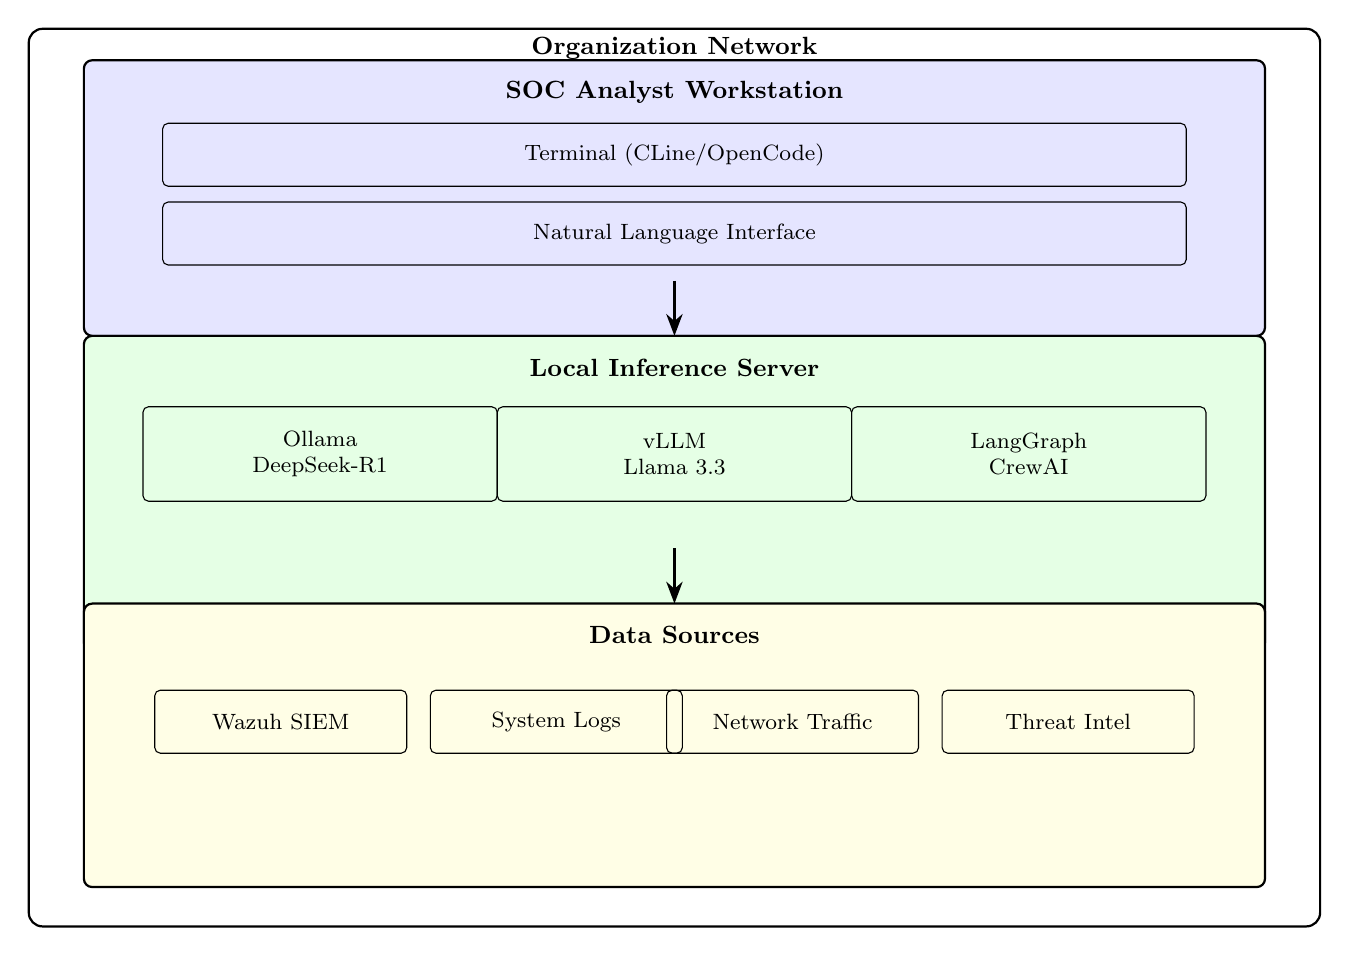
\begin{tikzpicture}[
  level/.style={draw, thick, rectangle, rounded corners=3pt, minimum width=16cm, align=center},
  subbox/.style={draw, rectangle, rounded corners=2pt, align=center, font=\footnotesize},
  arrow/.style={-{Stealth[scale=1.2]}, thick}
]

% ===== LEVEL 1: SOC Analyst Workstation =====
% Level background box (drawn first so it's behind everything)
\draw[thick, rounded corners=3pt, fill=blue!10] (-7.5, 0) rectangle (7.5, -3.5);
\node[font=\small\bfseries] at (0, -0.4) {SOC Analyst Workstation};

% Components inside Level 1
\node[subbox, minimum width=13cm, minimum height=0.8cm] at (0, -1.2) (term) {Terminal (CLine/OpenCode)};
\node[subbox, minimum width=13cm, minimum height=0.8cm] at (0, -2.2) (nlp) {Natural Language Interface};

% Arrow 1
\draw[arrow] (0, -2.8) -- (0, -3.5) coordinate(arrow1);

% ===== LEVEL 2: Local Inference Server =====
% Level background box
\draw[thick, rounded corners=3pt, fill=green!10] (-7.5, -3.5) rectangle (7.5, -7.5);
\node[font=\small\bfseries] at (0, -3.9) {Local Inference Server};

% Components inside Level 2
\node[subbox, minimum width=4.5cm, minimum height=1.2cm] at (-4.5, -5.0) (ollama) {Ollama\\DeepSeek-R1};
\node[subbox, minimum width=4.5cm, minimum height=1.2cm] at (0, -5.0) (vllm) {vLLM\\Llama 3.3};
\node[subbox, minimum width=4.5cm, minimum height=1.2cm] at (4.5, -5.0) (lang) {LangGraph\\CrewAI};

% Arrow 2
\draw[arrow] (0, -6.2) -- (0, -6.9) coordinate(arrow2);

% ===== LEVEL 3: Data Sources =====
% Level background box
\draw[thick, rounded corners=3pt, fill=yellow!10] (-7.5, -6.9) rectangle (7.5, -10.5);
\node[font=\small\bfseries] at (0, -7.3) {Data Sources};

% Components inside Level 3
\node[subbox, minimum width=3.2cm, minimum height=0.8cm] at (-5.0, -8.4) (wazuh) {Wazuh SIEM};
\node[subbox, minimum width=3.2cm, minimum height=0.8cm] at (-1.5, -8.4) (syslogs) {System Logs};
\node[subbox, minimum width=3.2cm, minimum height=0.8cm] at (1.5, -8.4) (net) {Network Traffic};
\node[subbox, minimum width=3.2cm, minimum height=0.8cm] at (5.0, -8.4) (ti) {Threat Intel};

% Outer bounding box - Organization Network
\draw[thick, rounded corners=5pt] (-8.2, 0.4) rectangle (8.2, -11.0);
\node[font=\small\bfseries] at (0, 0.15) {Organization Network};

\end{tikzpicture}
\caption{Deployment Architecture Diagram}
\label{fig:deployment}
\end{figure}


\section{Expected Outcome}

\subsection{Functional Outcomes}
\begin{itemize}
    \item Autonomous SOC agent with full CLI accessibility.
    \item Real-time detection: accuracy >95\%, false positive rate <10\%.
    \item Explainable alerts with SHAP/LIME justifications.
    \item Automated forensic reports (JSON/HTML) generated within 5 minutes.
    \item LLM-based decision support for cross-alert correlation.
    \item Unified pipeline: no manual handoffs between detection and forensics.
\end{itemize}

\subsection{Performance Outcomes}
\begin{table}[H]
\centering
\caption{Expected Performance Improvements}
\begin{tabular}{@{}lccc@{}}
\toprule
\hcell{Metric} & \hcell{Baseline (Manual)} & \hcell{Expected} & \hcell{Improvement} \\
\midrule
False Positive Rate & >90\% & <10\% & 80\%+ reduction \\
Alert Processing Time & 5--10 min & 10--30 sec & 90\%+ reduction \\
Mean Time to Detect & Hours--Days & Minutes & 95\%+ reduction \\
Mean Time to Respond & Hours--Days & Minutes--Hours & 80\%+ reduction \\
Analyst Workload & 100\% & 20--30\% & 70\%+ reduction \\
\bottomrule
\end{tabular}
\end{table}

\subsection{Deliverables}
\begin{itemize}
    \item \textbf{Software:} Complete source code, pre-trained CNN/LSTM models, Wazuh integration scripts, forensic modules, natural language terminal interface, Docker container.
    \item \textbf{Documentation:} Installation guide, user manual, API documentation, training materials.
    \item \textbf{Validation:} Test results on NSL-KDD, CICIDS2017; performance benchmarks; XAI explanation quality assessment; security/privacy validation report.
\end{itemize}

\subsection{Benefits}
\begin{itemize}
    \item \textbf{To SOC operations:} Automates 70--80\% of Tier~1 triage, reduces FPR by 80\%+, decreases MTTR from hours to minutes.
    \item \textbf{To analysts:} Eliminates repetitive triage, enables focus on threat hunting, serves as a learning tool.
    \item \textbf{To organizations:} Reduces need for large Tier~1 teams, lowers operational costs, strengthens security posture.
\end{itemize}

% ============================================================
% REFERENCES
% ============================================================
\chapter{References}
\begin{thebibliography}{99}

\bibitem{kersten2023} L. Kersten, T. Mulders, E. Zambon, C. Snijders, and L. Allodi, ``Give Me Structure: Synthesis and Evaluation of a (Network) Threat Analysis Process Supporting Tier 1 Investigations in a Security Operation Center,'' in \textit{Nineteenth Symposium on Usable Privacy and Security (SOUPS 2023)}, Anaheim, CA, USA, Aug. 2023, pp. 97-111.

\bibitem{vielberth2020} M. Vielberth, F. Böhm, I. Fichtinger, and G. Pernul, ``Security Operations Center: A Systematic Study and Open Challenges,'' \textit{IEEE Access}, vol. 8, pp. 227756-227779, 2020.

\bibitem{ban2021} T. Ban, N. Samuel, T. Takahashi, and D. Inoue, ``Combat Security Alert Fatigue with AI-Assisted Techniques,'' in \textit{Proceedings of the 14th Cyber Security Experimentation and Test Workshop (CSET '21)}, Virtual, CA, USA, 2021, pp. 9-16.

\bibitem{furnell2021} S. Furnell, ``The cybersecurity workforce and skills,'' \textit{Computers \& Security}, vol. 100, p. 102080, 2021.

\bibitem{sundaramurthy2015} S. C. Sundaramurthy, A. G. Bardas, J. Case, et al., ``A Human Capital Model for Mitigating Security Analyst Burnout,'' in \textit{Eleventh Symposium On Usable Privacy and Security (SOUPS 2015)}, Ottawa, Canada, Jul. 2015, pp. 347-359.

\bibitem{zhao2023} W. X. Zhao, K. Zhou, J. Li, et al., ``A Survey of Large Language Models,'' \textit{arXiv preprint arXiv:2303.18223}, 2023.

\bibitem{yao2024} Y. Yao, J. Duan, K. Xu, et al., ``A Survey on Large Language Model (LLM) Security and Privacy: The Good, The Bad, and The Ugly,'' \textit{High-Confidence Computing}, vol. 4, no. 2, p. 100211, 2024.

\bibitem{motlagh2024} F. N. Motlagh, M. Hajizadeh, M. Majd, P. Najafi, F. Cheng, and C. Meinel, ``Large Language Models in Cybersecurity: State-of-the-Art,'' \textit{arXiv preprint arXiv:2402.00891}, 2024.

\bibitem{kaheh2023} M. Kaheh, D. K. Kholgh, and P. Kostakos, ``Cyber Sentinel: Exploring Conversational Agents in Streamlining Security Tasks with GPT-4,'' \textit{arXiv preprint arXiv:2309.16422}, 2023.

\bibitem{ren2025} S. Ren and S. Chen, ``Large Language Models for Cybersecurity Intelligence, Threat Hunting, and Decision Support,'' \textit{IEEE Access}, vol. 12, pp. 1-20, 2025.

\bibitem{oniagbi2024} O. Oniagbi, ``Evaluation of LLM Agents for the SOC Tier 1 Analyst Triage Process,'' M.S. thesis, Dept. Computing, University of Turku, Turku, Finland, 2024.

\bibitem{fang2024} R. Fang, R. Bindu, A. Gupta, and D. Kang, ``LLM Agents can Autonomously Exploit One-day Vulnerabilities,'' \textit{arXiv preprint arXiv:2404.08144}, 2024.

\bibitem{karlsen2023} E. Karlsen, R. Copstein, X. Luo, et al., ``Exploring semantic vs. syntactic features for unsupervised learning on application log files,'' in \textit{2023 7th Cyber Security in Networking Conference (CSNet)}, IEEE, 2023, pp. 219-225.

\bibitem{wu2023} T. Wu, S. He, J. Liu, et al., ``A Brief Overview of ChatGPT: The History, Status Quo and Potential Future Development,'' \textit{IEEE/CAA Journal of Automatica Sinica}, vol. 10, no. 5, pp. 1122-1136, 2023.

\bibitem{salloum2025} M. Salloum and S. Norozpour, ``Explainable Artificial Intelligence for Cybersecurity Applications,'' \textit{IEEE Access}, vol. 13, pp. 69-80, 2025.

\bibitem{zieni2023} R. Zieni, L. Massari, and M. Calzarossa, ``Phishing or not phishing? A survey on the detection of phishing websites,'' \textit{IEEE Access}, vol. 11, pp. 18499-18519, 2023.

\bibitem{capuano2022} N. Capuano, G. Fenza, V. Loia, and C. Stanzione, ``Explainable artificial intelligence in cybersecurity: a survey,'' \textit{IEEE Access}, vol. 10, pp. 93575-93600, 2022.

\bibitem{lundberg2017} S. M. Lundberg and S.-I. Lee, ``A unified approach to interpreting model predictions,'' in \textit{Advances in Neural Information Processing Systems}, vol. 30, 2017, pp. 4768-4777.

\bibitem{ribeiro2016} M. T. Ribeiro, S. Singh, and C. Guestrin, ``Why should I trust you? Explaining the predictions of any classifier,'' in \textit{Proceedings of the 22nd ACM SIGKDD International Conference on Knowledge Discovery and Data Mining}, 2016, pp. 1135-1144.

\bibitem{aizpurua2024} B. Aizpurua, S. Palmer, and R. Orus, ``Tensor networks for explainable machine learning in cybersecurity,'' \textit{Neurocomputing}, vol. 600, pp. 1-10, 2024.

\bibitem{calzarossa2025} M. C. Calzarossa, P. Giudici, and R. Zieni, ``An assessment framework for explainable AI with applications to cybersecurity,'' \textit{Artificial Intelligence Review}, vol. 58, no. 150, pp. 1-19, 2025.

\bibitem{ankalaki2025} S. Ankalaki, A. R. Atmarkur, M. Pallavi, et al., ``Cyber Attack Prediction: From Traditional Machine Learning to Generative Artificial Intelligence,'' \textit{IEEE Access}, vol. 13, pp. 44652-44700, 2025.

\bibitem{rishad2025} S. M. S. Rishad, F. Shakil, S. A. Tisha, et al., ``Leveraging AI and Machine Learning for Predicting, Detecting, and Mitigating Cybersecurity Threats: A Comparative Study of Advanced Models,'' \textit{International Journal of Computer Science \& Information System}, vol. 10, no. 1, pp. 6-25, 2025.

\bibitem{alshurbaji2025} T. Al-Shurbaji, M. Anbar, S. Manickam, et al., ``Deep Learning-Based Intrusion Detection System for Detecting IoT Botnet Attacks: A Review,'' \textit{IEEE Access}, vol. 13, pp. 1-31, 2025.

\bibitem{hiari2025} M. Hiari, Y. Alraba'nah, and I. Qaddara, ``A Deep Learning-Based Intrusion Detection System using Refined LSTM for DoS Attack Detection,'' \textit{Engineering, Technology \& Applied Science Research}, vol. 15, no. 4, pp. 25627-25633, 2025.

\bibitem{ndihe2024} O. S. Ndihe, ``AI-Driven Forensic Systems for Real-Time Anomaly Detection and Threat Mitigation in Cybersecurity Infrastructures,'' M.S. thesis, University of Central Missouri, USA, 2024.

\bibitem{kolluri2016} V. Kolluri, ``A pioneering approach to forensic insights: Utilization AI for cybersecurity incident investigations,'' \textit{IJRAR-International Journal of Research and Analytical Reviews (IJRAR)}, vol. 3, no. 3, pp. 1-10, 2016.

\bibitem{kara2023} I. Kara, ``Fileless malware threats: Recent advances, analysis approach through memory forensics and research challenges,'' \textit{Expert Systems with Applications}, vol. 214, p. 119133, 2023.

\bibitem{rana2025} M. Rana, ``Enhancing Zero Trust Cybersecurity with AI,'' \textit{Journal of Information Systems Engineering Management}, vol. 10, no. 32s, pp. 1-6, 2025.

\bibitem{chen2024} W. Chen, Y. Zhang, X. Liu, et al., ``IntelliBot: retrieval augmented LLM chatbot for cyber threat knowledge delivery,'' \textit{arXiv preprint arXiv:2411.08234}, 2024.

\bibitem{muzsai2024} L. Muzsai, D. Imolai, and A. Lukacs, ``HackSynth: LLM agent and evaluation framework for autonomous penetration testing,'' \textit{arXiv preprint arXiv:2412.01778}, 2024.

\end{thebibliography}

\end{document}